\lecture{3}{Jan 24 01:10}{}
\section{Infinite Square Well}
\begin{remark}
    
We will solve for a case called the infinite square well. We can write the potential to be
\[
    V(x) = \begin{dcases}
        \infty , &\text{ if } x< 0  ;\\
        \infty , &\text{ if } x>a ;\\
        0, &\text{ otherwise} .
    \end{dcases}
\]
\[
    E \psi  = \frac{-\hbar ^{2} }{2m} \left[ \frac{\mathrm{d}^{2} \psi }{\mathrm{d}x^{2} }  \right] 
\] 
The solutions we have here are going to be 
\[
    A_0 = e^{\pm ikx}, k = \sqrt{\frac{2mE}{\hbar ^{2} }} 
\]
\begin{figure}[H]
    \centering
    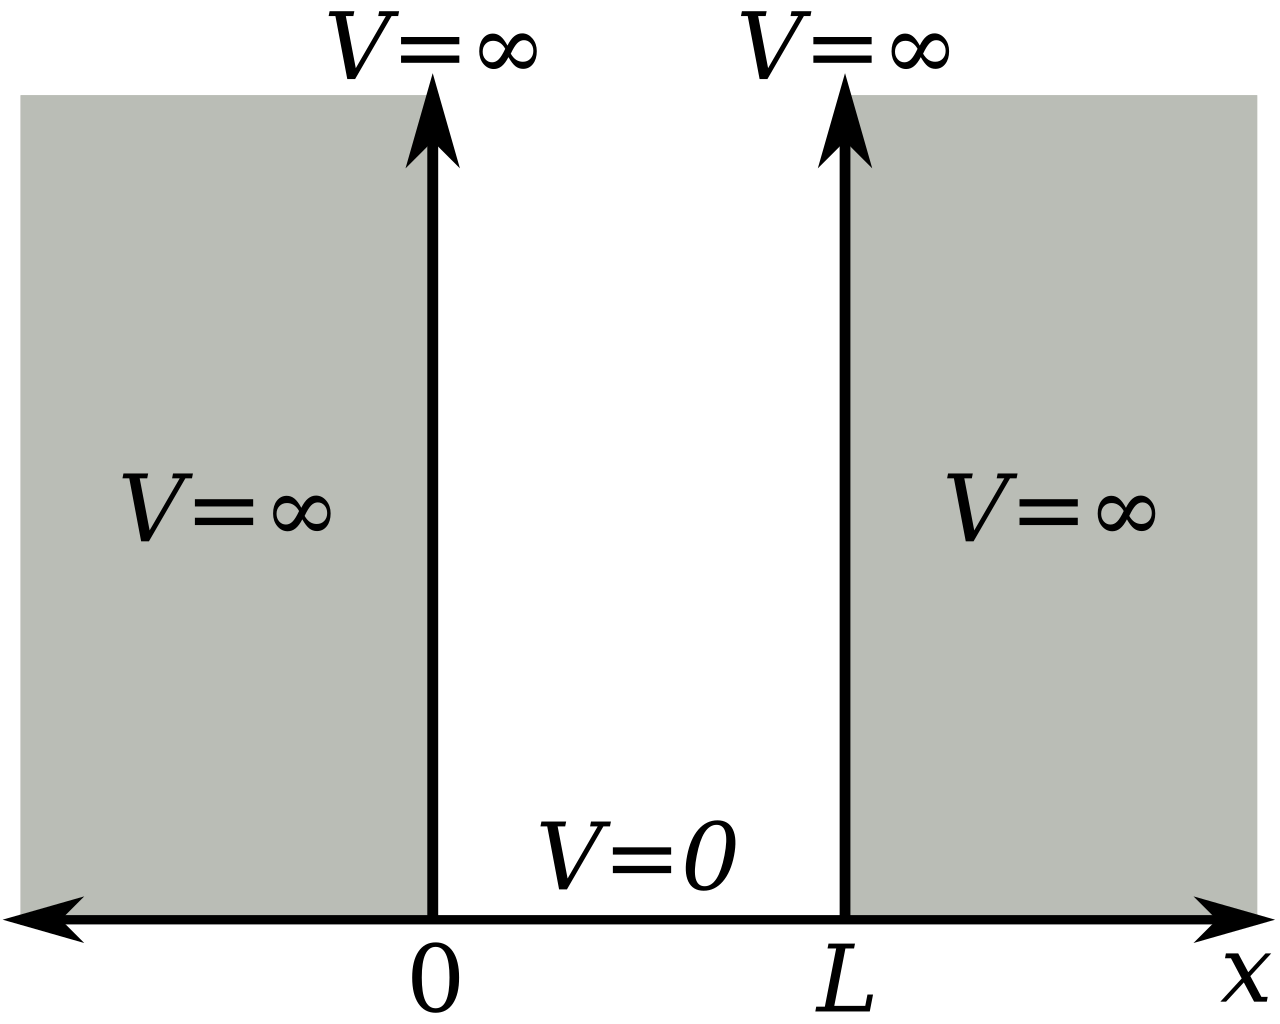
\includegraphics[width=0.5\textwidth]{Figures/kpZUe.png}
    \caption{}
    \label{fig:}
\end{figure}
Recall that we have the equation 
\[
    \psi  = Ae^{\alpha x} 
\]
\[
     -\left[ A \alpha ^{2}  e^{\alpha x} \right] \frac{\hbar ^{2} }{2m}\ = Ex
\]
\[
    -\frac{\hbar ^{2} \alpha ^{2} }{2m} = E
\]
\[
    \alpha ^{2}  = \frac{2mE}{\hbar ^{2} } \to  \alpha  = \pm i \sqrt{\frac{2mE}{\hbar ^{2} }} 
\]
\end{remark}
\begin{remark}
    Second Order Differential Equation:
    \[
        \psi  = A \sin (kx) + B \cos (kx)
    \]
    Note that \(\sin (kx) = \frac{e^{ikx} - e^{-ikx}  }{2}\) and \(\cos (kx)\) to have a positive term. We notice
    that immediately that the \(\cos (kx)\) term cannot be in the solution since the potential is \(V(0) = 0\) . 

    \[
        \psi  = A \sin  (kx)
    \]
    with an additional constraint that 
    \[
        \psi (x=a) = 0
    \]
    \[
        A\sin (ka) = 0 
    \]
    \[
        ka =  n\pi , k = \frac{n\pi}{a}
    \]
    There are only quantized values of \(k\) which means that the energy is also quantized where 
    \[
        E = \frac{\hbar ^{2}  k^{2} }{2m}
    \]
    \[
        E_n = \frac{\hbar ^{2}  \pi ^{2} }{2ma^{2}} n^{2} 
    \]Thus quantized energy states come from boundary conditions which lead to quantized energies. For free particles, 
    energy is continuous but as we put boundary conditions, energy is discretized. 
    \begin{figure}[H]
        \centering
        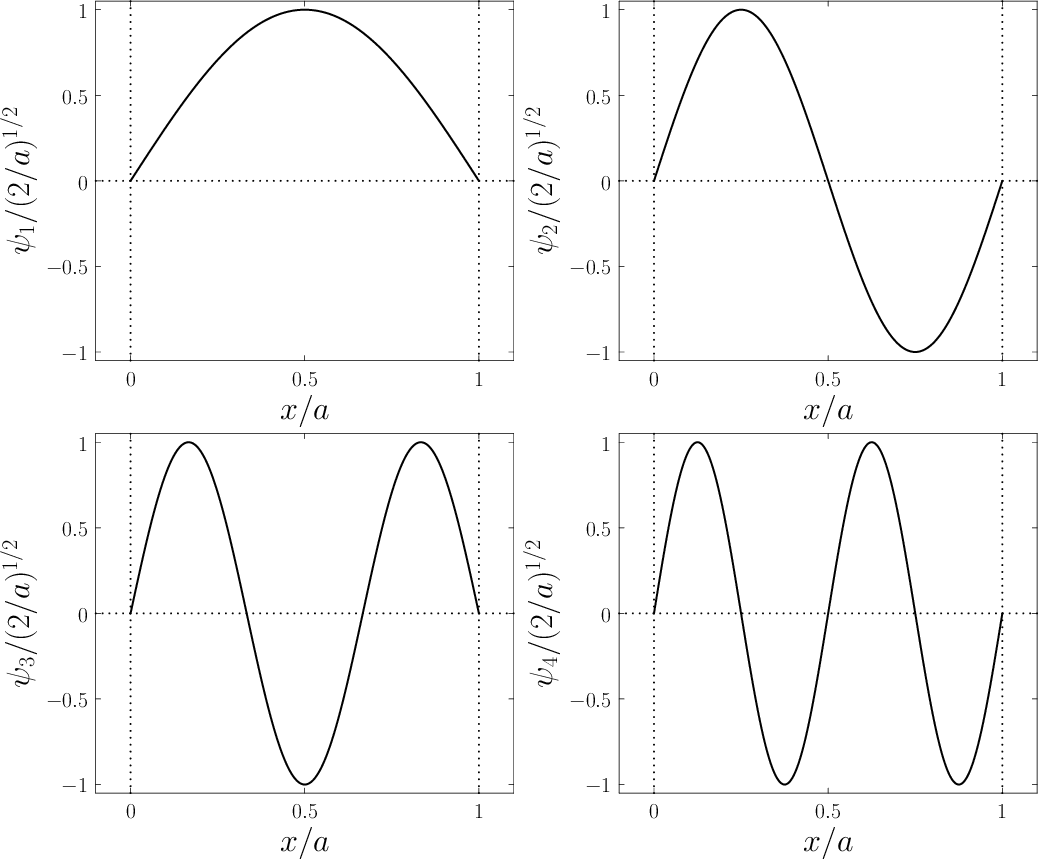
\includegraphics[width=0.8\textwidth]{Figures/img3046.png}
        \caption{}
        \label{fig:}
    \end{figure}
    These are the solutions for \(n=1,2,3,4\) where we see an additional oscillation for each term. 
\end{remark}
\begin{eg}
    For a given example, suppose we had a potential with 6 zeroes for our \(\psi \) , then our energy can be approximated to be 
    \[
        E \approx \frac{\hbar ^{2}  \pi ^{2} }{2ma^{2}} \times 5^{2} 
    \]
    \begin{figure}[H]
        \centering
        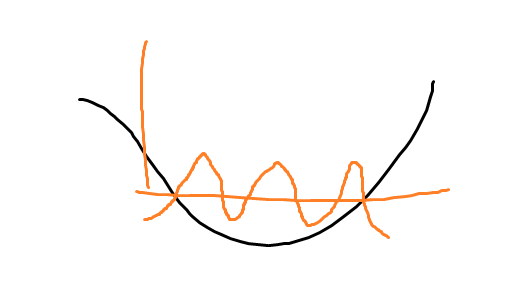
\includegraphics[width=0.8\textwidth]{Figures/01.png}
        \caption{}
        \label{fig:}
    \end{figure}
\end{eg}
\begin{remark}
    
Notice that we have been carrying a value \(A\), we most normalize to calculate expectation values. We normalize through 
the L2 norm which is given by 
\[
    \int_{-\infty}^{\infty} \vert \psi (x) \vert  ^{2} \,\mathrm{d}x  = 1 
\]
One nice thing about the infinite square welll is that it is finite. thus we have 
\[
    \int_{0}^{a}  A_n ^{2}  \sin ^{2} (\pi \frac{n}{a} x)\,\mathrm{d}x = 1
\]
We can redefine the argument and rescale giving a unitless integral. 
\[
    y= \pi \frac{n}{a} x, \mathrm{d}y  = \pi \frac{n}{a}\mathrm{d}x , 
\]
where \(y\) is a unitless term.  
\[
    A_n ^{2}  \frac{a}{n \pi } \int_{0}^{n \pi } \sin ^{2} (y)  \,\mathrm{d}y  = 1 
\]
\[
  \at{  A_n ^{2}  \frac{a}{n \pi } \left[  \frac{1}{2} (y-\sin (y)\cos (y))\right]}{0}{n \pi } = 1
\]
\[
    A_n ^{2}  \frac{a}{n \pi } \frac{1}{2} n \pi  = 1
\]
\[
    A_n ^{2}  = \frac{2}{a}
\]
\[
    A_n = \sqrt{\frac{2}{a}} 
\]
Thus, all normalized wave functions look like the following:
\[
    \psi _n (x) = \sqrt{\frac{2}{a}} \sin (\pi \frac{nx}{a})
\]
Notice that the time dependence is simply a separation of variables where 
\[
    \Psi (x,t) = \psi_n (x) \phi_n  (t)
\]
where 
\[
\phi _n (t) = e^{-iE_{n}\frac{t}{\hbar } } 
\]
Any expectation value we look at will be invariant with time. Notice that 
\[
    e^{-i\frac{E_n}{\hbar }t} = \cos (\frac{E_n}{\hbar }t) - i \sin (\frac{E_n}{\hbar }t) 
\]

\end{remark}
\begin{remark}
    Superposition: 
\[
    \psi (x,t) = \frac{1}{\sqrt{2} } \sqrt{\frac{2}{a}} \left[ \sin (\pi \frac{x}{a}) + \sin (2\pi \frac{x}{a})\right] 
\]
This is the solution at \(t=0\) where it is the superposition of the \(n = 1\) and \(n = 2\) solution. Suppose that 
we did not have the \(\frac{1}{\sqrt{2} }\) part, we would need to normalize. 
\[
     \psi  = C \sqrt{\frac{2}{a}} \left[ \psi _1 + \psi _2 \right] 
\] 
which is an equally waited superposition. We can normalize now with 
\[
    \int_{0}^{a}  \vert \psi \vert ^{2} \,\mathrm{d}x = \vert C \vert  ^{2}  \frac{2}{a} \int_{0}^{a}  \left[ \vert \psi _1 \vert  ^{2}  + \vert \psi _2 \vert ^{2}  + \psi_1^* \psi _2 + \psi _1 \psi _2 ^*\right] \,\mathrm{d}x 
\]
The only contribution will come from the absolute value terms.   Coming back we can write 
\[
    \psi_n (x,t) = \frac{1}{\sqrt{a} } \left[ \psi _1 (x) e^{-\frac{iE_1}{\hbar }t} + \psi _2 (x) e^{-\frac{iE_2}{\hbar }t}   \right] 
\] 
We will pick up when we have two stationary states in a infinite square well. We will end up getting some in phase and out of 
phase which will lead to varying time dependent argument presented here. 
\end{remark}
